\chapter{Background}\label{chap:background}
In this chapter we will define important terms and lay out the theoretical background for the remainder of the thesis.

\section{Definition of terms}
\paragraph{Citation} The term \emph{``citation''} can refer to both the act of citing as well as the occurrence of being cited. This can be illustrated with the phrase \emph{``an author's citations''}. In \cite{Beel2016} Beel et al. write \emph{``McNee et al. assumed that an author's citations indicate a positive vote for a paper [93].''} (the author cites), while Myers~\cite{Myers1970} writes \emph{``Thus, the number of an author's citations, in this study, means the number of articles in which one or more of his publications were cited.''} (the author is being cited). Like the latter example we will make an effort to use the term unambiguosly.
% also: \cite{Beel2016} \emph{``a few articles gained many citations (the maximum was 528 citations for [43]) and many articles had few citations, see Fig. 3.''} -> passive
\paragraph{Citation marker} A citation marker is a string of text that identifies an entry within a document's reference section. Examples are ``[27]'', ``[Bol98]'' and ``(He, 2010)''. These are placed within the document whenever the author refers to one of the documents in the reference section.
\paragraph{Citation context} The context of a citation is the text surrounding its citation marker. Typical sizes are 1--3 sentences. The sentence containing the marker is also sometimes referred to as ``citing sentence''. 

\begin{table}
\centering
    \caption[Examples of citations and their categorization into integral/non-integral as well as syntactic/non-syntactic.]{Examples of citations and their categorization into integral/non-integral (values left of split) as well as syntactic/non-syntactic (values right of split).}
    \label{tab:integralsyntactic}
\begin{center}
    \begin{tabular}{llllll|ll}%m{8cm}
    \toprule
    Context excerpt (citation marker {\color{UniBlue}highlighted}) & \rotatebox{90}{Swales~\cite{Swales1990}} & \rotatebox{90}{Hyland~\cite{Hyland1999}} & \rotatebox{90}{Thompson~\cite{Thompson2001}} & \rotatebox{90}{Okamura~\cite{Okamura2008}} & \rotatebox{90}{Lamers et al.~\cite{Lamers2018}} & \rotatebox{90}{Whidby et al.~\cite{Whidby2011}} & \rotatebox{90}{Abujbara et al.~\cite{Abujbara2012}} \\
    \midrule
    ``Swales {\color{UniBlue}(1990)} has argued that ...''                 & i & i & i & i & i & n & ? \\
    ``{\color{UniBlue}Swales (1990)} has argued that ...''                 & i & i & i & i & n & s & s \\
    ``Swales {\color{UniBlue}[42]} has argued that ...''                   & i & i & i & i & i & n & n \\
    ``Swales has argued that ... {\color{UniBlue}[42]}''                   & i & i & i & i & i & n & n \\
    ``It has been argued {\color{UniBlue}(Swales, 1990)} that ...''         & n & n & n & n & n & n & n \\
    ``It has been argued {\color{UniBlue}[42]} that ...''                  & n & n & n & n & n & n & n \\
    ``According to {\color{UniBlue}(Swales, 1990)} it is ...'' & ? & ? & ? & ? & n & s & s \\
    ``According to {\color{UniBlue}[42]} it is ...''          & n & n & n & n & n & s & s \\
    ``... has been shown (see {\color{UniBlue}(Swales, 1990)}).''           & n & n & n & n & n & s & n \\
    \bottomrule
    \end{tabular}
\end{center}
\end{table}

\paragraph{Integral and syntactic citations} There are two somewhat similar, and at first glance easily confused notions condsidering a citation's role within its context. They are referred to as ``integral''---in the adjectival sense close in meaning to ``essential'' or ``inherent'', not what we denote in caluclus with $\int$---and ``syntactic''. Integral citations were first defined by Swales~\cite{Swales1990} in 1990 and are a frequently used~\cite{Hyland1999,Thompson2001,Okamura2008,Lamers2018} measure in discourse analysis. An integral citation is, in Swales' own words, \emph{``one in which the name of the researcher occurs in the actual citing sentence as some sentence-element''}. Thompson~\cite{Thompson2001} rephrases the definition as \emph{``citations that [...] play an explicit grammatical role within a sentence''}. While what Thompson refers to as ``citations'' might be confused with the notion of citation markers, the examples given in \cite{Thompson2001} clearly indicate that a ``citaion'' is to mean an author's name in their definition. The second notion, ``syntactic'' (as used in \cite{Whidby2011} and \cite{Abujbara2012}), is concerned with whether or not a \emph{citation marker} has a grammatical role within its context. In other words, if removing the citation marker would make the citing sentence ungrammatical, then it is syntactic. Table~\ref{tab:integralsyntactic} gives an overview of examples for both concepts. Note that Lamers et al.~\cite{Lamers2018} provide a classification algorithm for integral and non-integral citations that slightly differs from Swales' original definition depending on the interpretation of a citation marker's scope, but also gives a clear classification in an edge case where Swales's definition is unclear. Furthermore note that the the two ways for distinguishing syntactic and non-syntactic citations found in literature are not identical. This is in part because the method given in \cite{Abujbara2012} is kept rather simple. For the intents and purposes of this work we can follow the definitions of Lamers et al. and Whidby et al. for ``integral'' and ``syntactic'' respectively.
\paragraph{Reference} References are the entries in a document's reference section. Each reference should unambiguously identify another document that it points to. In the context of parsing reference sections we will, at times, refer to references as ``reference strings''. An example of a reference is \emph{``W. Huang, P. Mitra, and C. L. Giles, `RefSeer: A citation recommendation system,' in IEEE/ACM Joint Conference on Digital Libraries, pp. 371–374, Sep. 2014.''}.
\paragraph{Reference resolution} The act of parsing a reference string and matching it to a document identifier is what we refer to as ``reference resolution''. Examples can be found in Section~\ref{sec:refresol}.
% \paragraph{Citation recommendation} global/local  % already explained in first chapter
\paragraph{Named Entity} In natural language processing the term ``Named Entity'' (NE) describes unambiguous abstract or physical entities which have a proper name. Examples are people (Tim Berners-Lee), places (the city Taipei), organizations (the Free Software Foundation) and concepts (Okapi BM25). For a more detailed discussion of the term see~\cite{Nadeau2007}.
\paragraph{Noun phrase} A noun phrase is a group of words (or a single word) functioning grammatically as one unit, that has a noun at its head. Examples are ``\emph{example}'', ``noun \emph{phrase}'' and ``context-based co-citation \emph{recommendation}'' (head of the phrase \emph{highlighted}).
\paragraph{Claim} For the scope of this thesis we define a ``claim'' as a verifiable statement in writing. The motivation for this definition is to capture those parts of publications, that are backed by citations. Examples are ``CiteSeer was introduced in 1998.'' and ``Parsing \LaTeX{} sources is a non trivial task.''.
\paragraph{Citation recommendation} We define ``citation recommendation'' as the task of recommending publications for purpose of referencing them. The input for a recommendation is at least a citation context (optionally more, like information on the author) and the output a list of publications that can or should be referred to from within the context. To give an example, a good recommendation for the input ``CiteSeer was introduced in 1998.'' would be ``K. D. Bollacker, S. Lawrence, and C. L. Giles, \emph{`CiteSeer: An Autonomous Web Agent for Automatic Retrieval and Identification of Interesting Publications'}, AGENTS `98''.

\section{Theoretical background}
\subsection{Recommending scientfic publications}
Generally speaking, recommender systems are tools of discovery. In situations where a user can not reasonably be assumed to consider all availabe options, a recommender system's task is to identify those items that maximize a user's satisfaction, service provider's revenue or similar goal. This is typically done by calculating a score for each available item, ranking them by score and finally presenting the top ones to the user. Common domains of recommendation are shopping products and media (movies, news articles, etc.). A coarse distinction of techniques for recommendation---ignoring hybrid and less conventional cases---can be made between \emph{content-based} and \emph{collaborative filtering}. The latter exploits the similarity of user profiles for recommendation, while the former operates on the similarity of the items.~\cite{Ricci2015}

Scientific publications as a recommender domain has some atypical characteristics. One of these is the ratio of users to items. Comparing, for example, to movie recommendation, the average number of new movies listed on the Internet Movie Database (IMDb) for the last 10 years (2009--2018) is about the same as the average number of new publications in the field of high energy physics on arXiv.org for the same time span---about 9,500 new items per year in both cases. Needless to say, there is more people watching movies than doing research in high energy physics. This can mean fewer users to compare to, when using collaborative filtering methods to recommend scientfic publications. Another peculiarity in this domain is the interconnectedness of items. While movies may have aspects like actors, directors, locations, etc. in common, scholarly writings not only share authors, venues, journals, etc. but are furthremore interconnected through citations. A consequence of this is the feasibility to utilize citation networks and citation contexts for recommendation.

Recommendation of scientfic publications can be done for several purposes, like introducing researchers to papers they might want to read, identifying works that are relevant to a draft of a new paper or suggesting publications that can be cited in a given context. While in all of these cases the nature of the items remains the same, input and constraints for the recommendation process differ. For the discovery of papers a researcher might find worthwihle reading, the focus lies on the researchers interest and there are no externally imposed hard constraints. In contrast, when recommending publications for the use of citation, the context of the citation plays a considerably larger role than an author's interest. There might be some leeway for personal citation style, but by and large the adequacy of a citation is dictated by its target context and the contents of candidate items. In this way, the task of citation recommendation can also be seen as a more general information retrieval problem where the citation context is the query for which adequate citations have to be identified.

Having established the relative position of the field of citation recommendation with respect to related fields, we will lay out the core concepts relevant to our approach, \emph{content based local citation recommendation by use of citation contexts}, below.

\begin{figure}
  \centering
    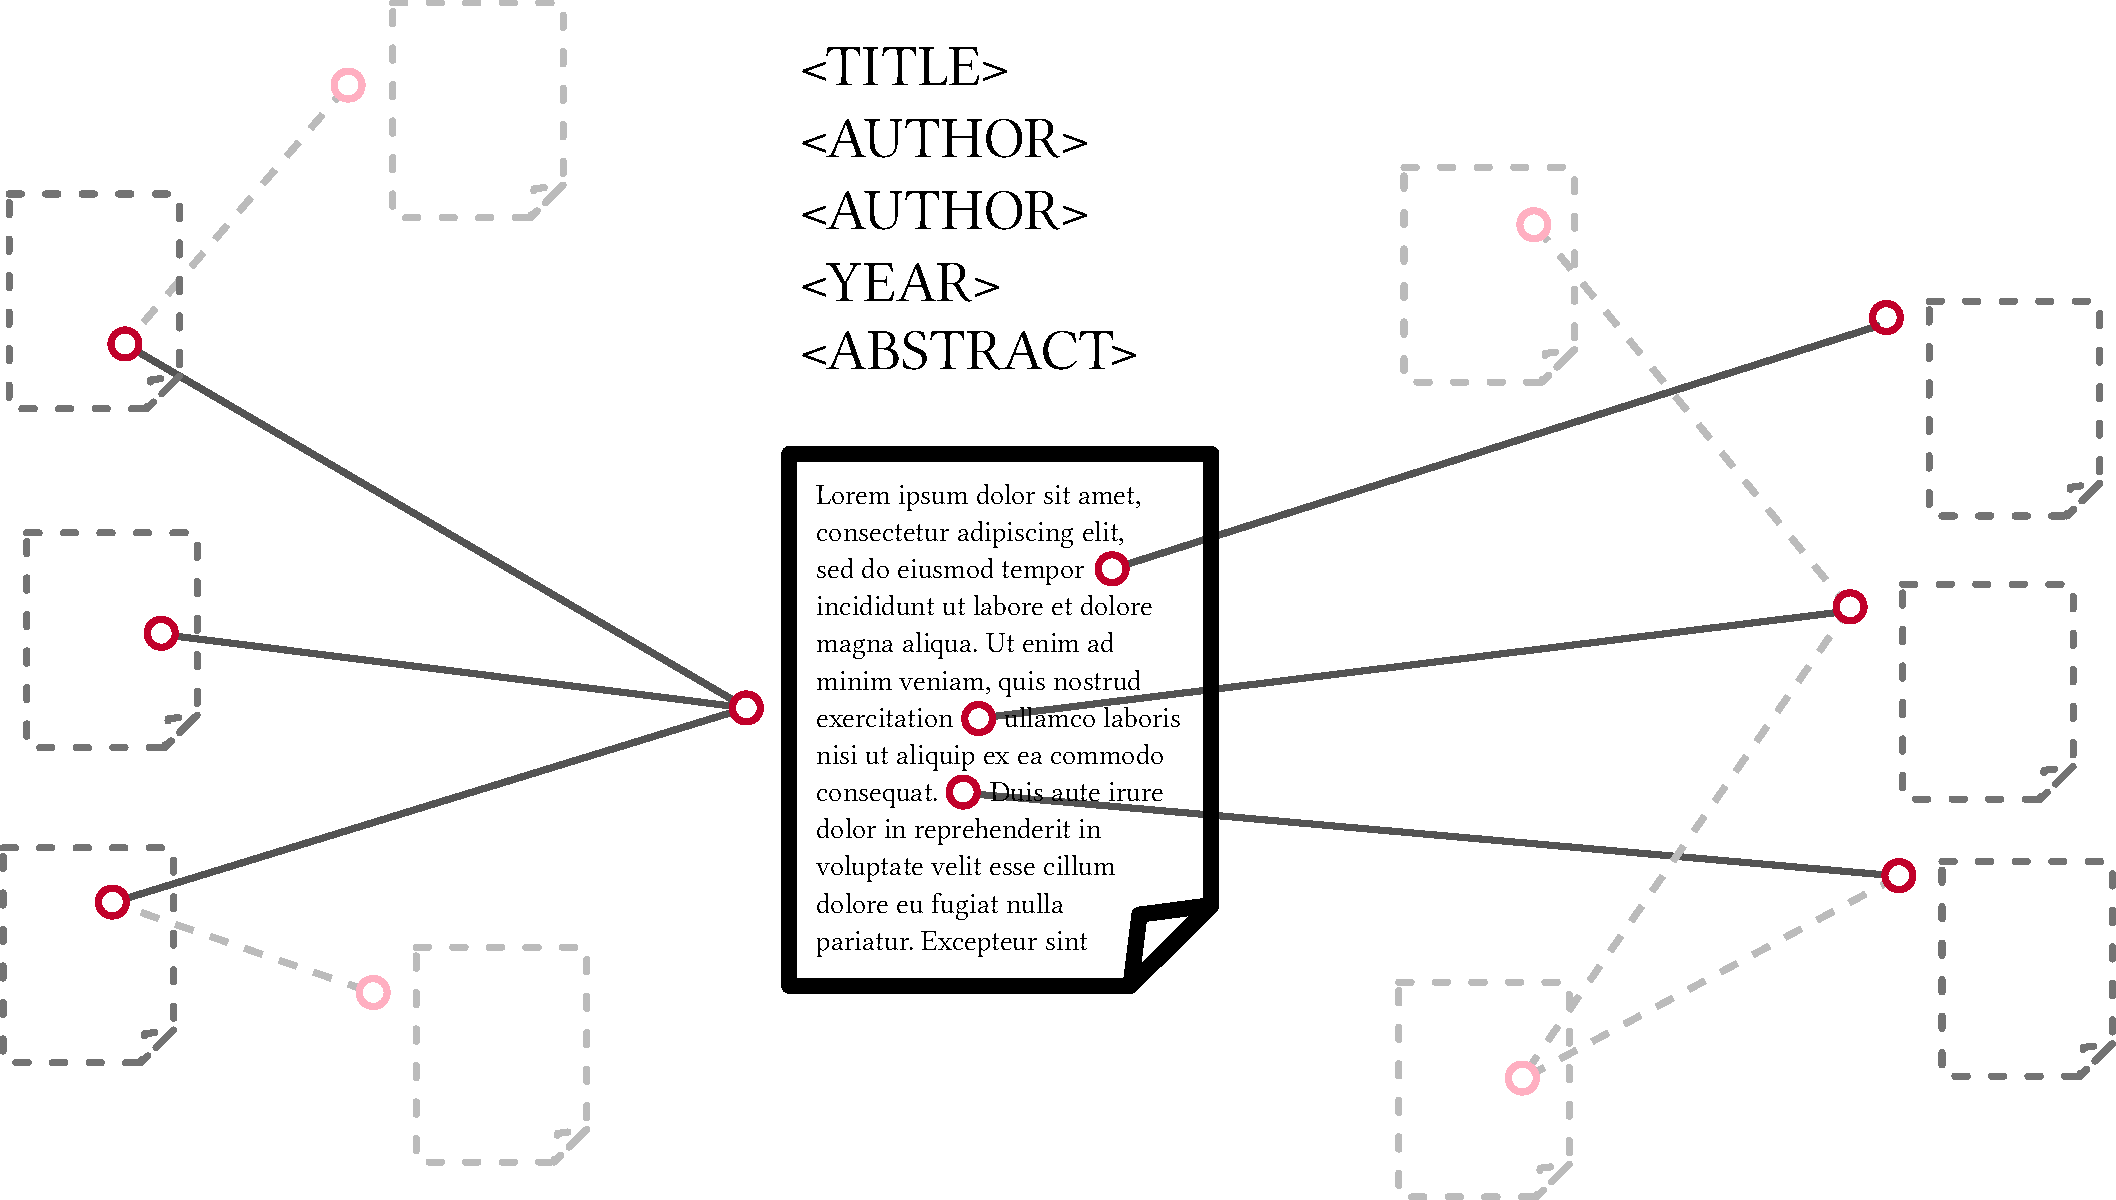
\includegraphics[width=0.8\textwidth]{figures/background/document_rich_view.pdf}
  \caption{Schematic view on a document, its metadata and embedding in the citation graph.}
  \label{fig:docrichview}
\end{figure}

\begin{figure}[t]
  \centering
    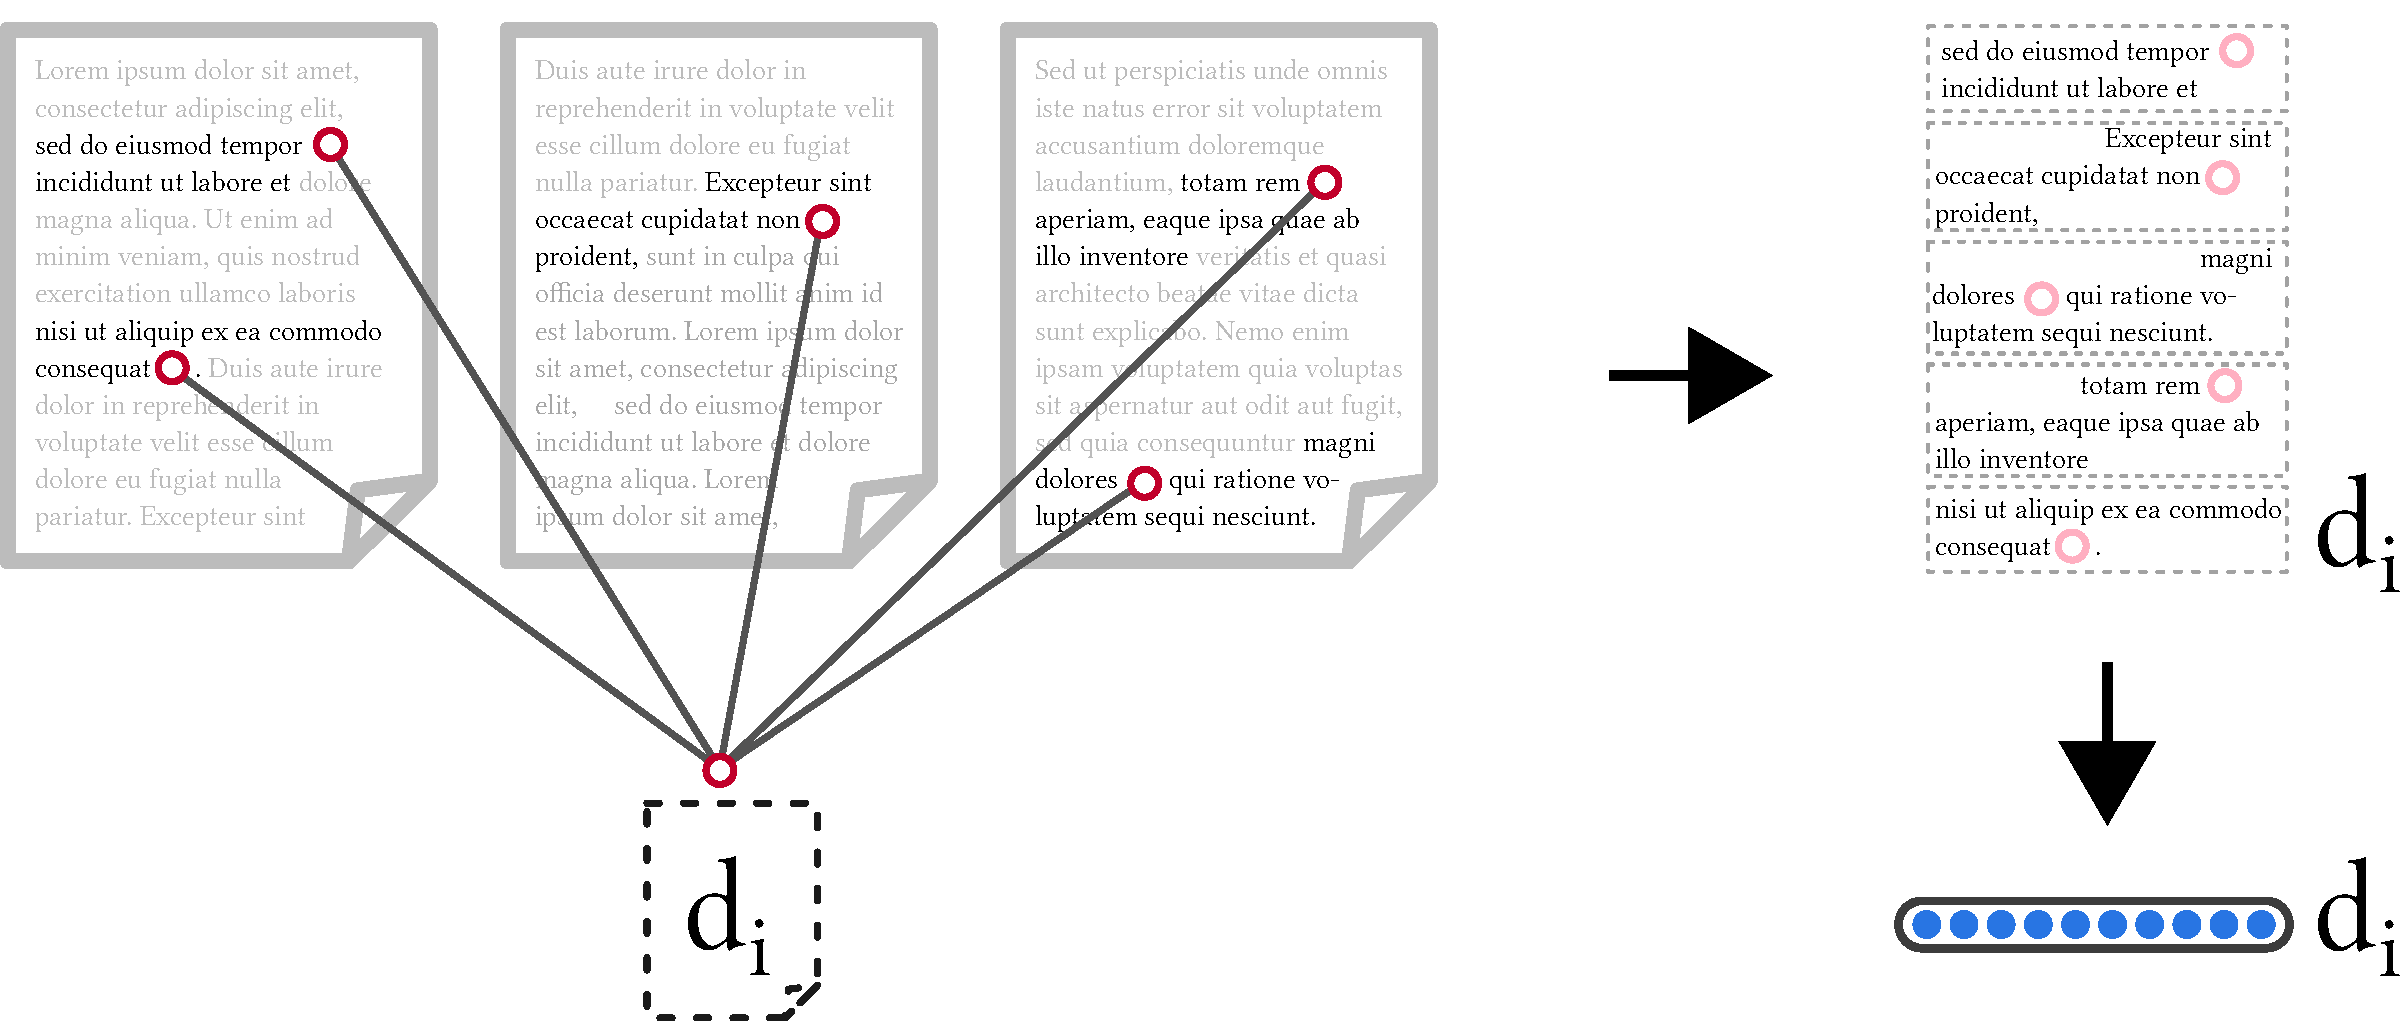
\includegraphics[width=\textwidth]{figures/background/document_context_view_withvec.pdf}
  \caption{Schematic visualization of a document's representation using citation contexts.}
  \label{fig:doccontview}
\end{figure}

As mentioned above, the focus in the case of citation recommendation lies on the candidate items---which are scientific publications. Figure~\ref{fig:docrichview} shows the types of information that are available to describe them. First and foremost each publication has, of course, its textual contents. Alongside this it is also part of a network of citations, meaning is has documents it is being cited by as well as documents it is citing. Lastly, there may also be metadata describing the document, such as the title, authors, year of publication etc. In order to study the viability of using explicit semantic representations of citation contexts for citation recommendation, without introducing any confounding variables, we will describe our documents \emph{only} by citation contexts. As citation contexts have been shown to contain information similar to and sometimes more extensive and focussed than abstracts~\cite{Elkiss2008}, we can expect decent recommendation results even though we're not taking any metadata associated with or textual content contained in the candidate documents into account. Figure~\ref{fig:doccontview} shows how a document representation can be generated from citation contexts. Document $d_i$ is cited by several other documents. By aggregating the contexts of these citations and deriving an abstract representation, $d_i$ can be represented by how it is being referenced in existing literature.
% Generating such representations of recommendation candidates is referred to as learning or training.

\begin{figure}[!b]
  \centering
    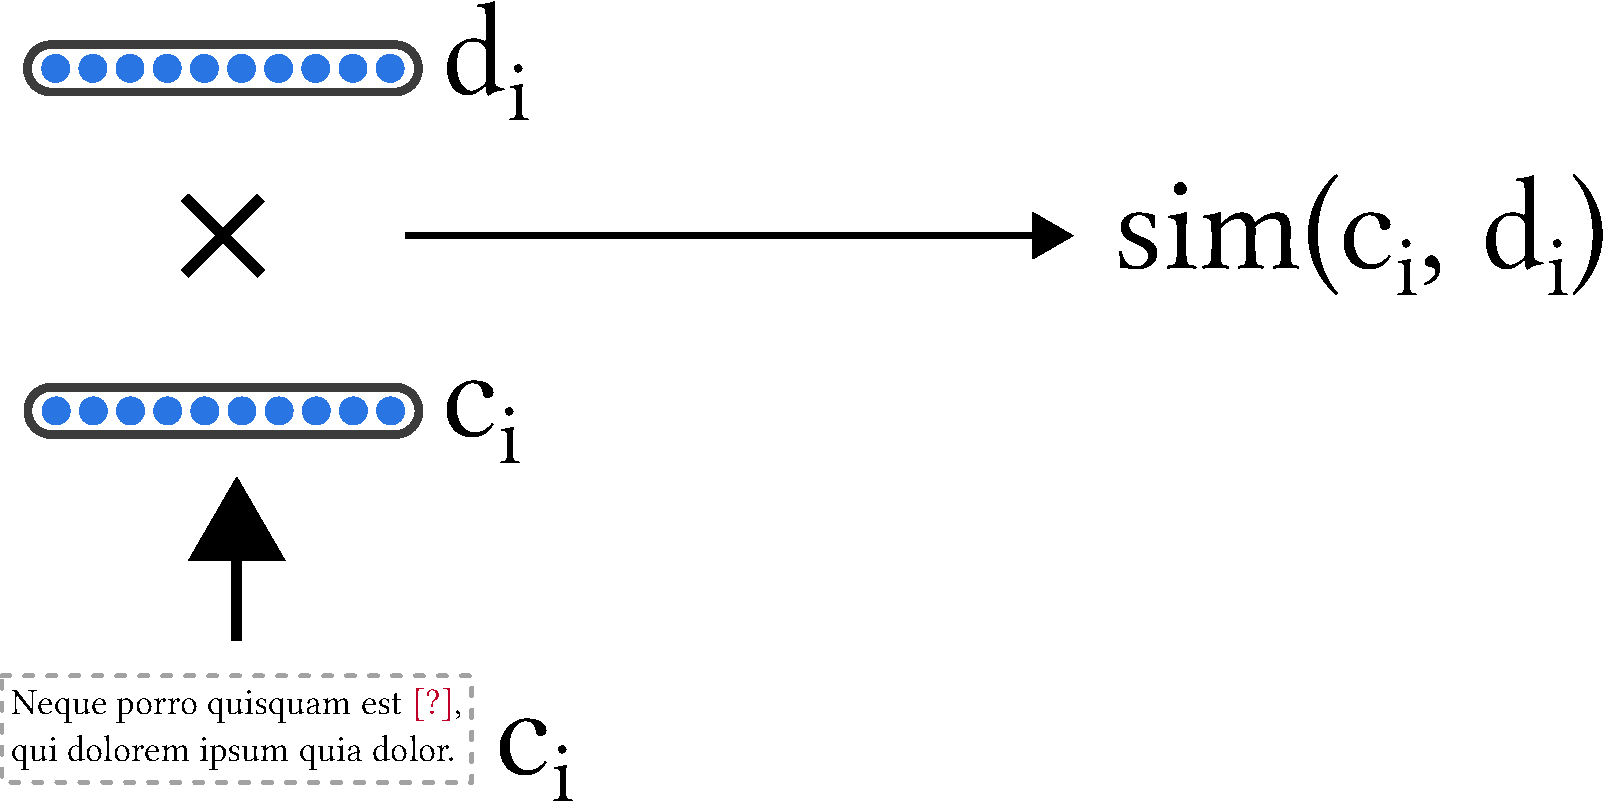
\includegraphics[width=0.7\textwidth]{figures/background/document_context_view_comparison.pdf}
  \caption{Schematic visualization of determining the similarity between an input citation contexts and a document representation.}
  \label{fig:doccomp}
\end{figure}

Recommendation itself is then done by taking a citation contexts $c_i$ as input, deriving an abstract representation in the same manner as was done for the aggregated contexts referencing a document, and then comparing the input's representation against those of all the documents. One such comparison is schematically depicted in Figure~\ref{fig:doccomp}. When every document---i.e., recommendation candidate---is associated with a similarity score, the system can output the most similar candidates as recommendations. With this, the overall picture looks as follows. The recommender system is trained on citation contexts, from which representations of the cited documents are learned. These documents are the publications the system is able to recommend. For a new context (without attached citation) given as input, the system identifies the documents most similar in the abstract representation space to the input and outputs these as recommendations.

\subsection{Evaluating citation recommendations}
Evaluation of recommender systems can be diveded into three types, online evaluation, user study and offline evaluation. Online evaluation refers to monitoring naturally occuring user interaction with a system deployed online and drawing conclusions from metrics like click-through rates. User studies are conducted in a more controlled manner where users are aware of the evaluation and may be asked for explicit feedback on parts of the system. Offline evaluation differs from the other two types in that it does not directly involve human judgement. Rather, part of the data the system would, for online deployment, be trained on, is withheld and used as testing data. In doing this, past user judgement (like rating a movie or placing a citation) is used as a ground truth to test the system's output against. Because the human judgement is implicitly given within the data and can be processed automatically, offline evaluations can easily be performed on a large scale.~\cite{Aggarwal2016}

When recommending citations, abovementioned three types of evaluation can be realized as follows. Online evaluation can be performed by measuring which, if any, of the suggested publications a user actually inserts into their text. In a user study, participants can be asked to judge the relevance of recommended items while the system's input could be chosen by the user or given by the creators of the study. Lastly, offline evaluation as outlined above results in a re-prediction setting. That is, existing citation contexts are stripped of their citations, input into the system, and the resulting output compared to the original.

To aggregate relevance judgements of a large number of recommendations into a single number in order to compare different approaches, metrics are necessary. We use Recall, MRR, MAP and NDCG measured at different cut-off values. A cut-off, often denoted as \emph{Metric@}$k$, means only taking the top $k$ recommendations into consideration. This is done because, realistically, a user will not go through a list of hundreds of suggested items, but only look at the top three, five or maybe ten. Recall, MRR, MAP and NDCG with a cut-off $k$ can be defined as follows (see \cite{Aggarwal2016} for a more detailed, general discussion of these metrics):

Let $\mathcal{R} = r_1,r_2, ..., r_n$ be the ordered list of recommended items (highest to lowest) and ${\mathit{rel}(r_i)\in[0, 1]}$ denote the relevance of item $r_i$ at rank $i$. Furthermore let ${\mathcal{R}_{rel}=\{r_i|\mathit{rel}(r_i)=1\}}$ be the set of relevant items in an evaluation where $\mathit{rel}(r_i)\in\{0,1\}$---that is, an item is either relevant or not, with no partial relevance inbetween. Note that in a re-prediction setting as described above, $|\mathcal{R}_{rel}|=1$.

\paragraph{Recall} measures the fraction of the number of relevant items that was retrieved. If a cut-off $k$ is applied, the fraction's denominator is the minimum of the number of relevant items and the cut-off value.\[ \mathit{Recall}@k = \frac{\sum\limits_{i=1}^{k} \mathit{rel}(r_i)}{\mathit{min}(|\mathcal{R}_{rel}|,k)} \] For an evaluation with multiple test inputs, the mean over all Recall@k values is taken.

\paragraph{MRR} (mean reciprocal rank) is a metric often used when there is just one relevant item (e.g. re-prediction of a citation). It takes into account the position of a recommended item through dividing its relevance by its rank.\[ \mathit{MRR}@k = \frac{\sum\limits_{i=1}^{k} \frac{\mathit{rel}(r_i)}{i}}{\mathit{min}(|\mathcal{R}_{rel}|,k)} \] Again, when evaluating over multiple test inputs, the mean over all MRR@k values is calculated.

\paragraph{MAP} (mean average precision) is the mean of average precision (\textbf{AP}) values of multiple queries. AP measures the average of all precision values at the ranks where relevant items are found. To define this, let $\rho(k)$ denote the number of relevant items within the first $k$ ranks. AP is then defined as \[ \mathit{AP}@k = \frac{\sum\limits_{i=1}^{k} \frac{\rho(i)}{i}\times\mathit{rel}(r_i)}{\mathit{max}(\rho(k), 1)} \] where $\mathit{rel}(r_i)\in\{0,1\}$. The value of MAP@k is the mean AP@k over all evaluated queries.

\paragraph{NDCG} (normalised discounted cumulative gain) is a metric compatible with non-binary relevance values that, similar to MAP, places higher weight on top ranks. It is calculated as the DCG (discounted cumulative gain) over the IDCG (ideal discounted cumulative gain)
 \[ \mathit{NDCG}@k = \frac{DCG@k}{IDCG@k} \]
where DCG is a sum of discounted relevance values
 \[ \mathit{DCG}@k = \sum\limits_{i=1}^{k} \frac{2^{\mathit{rel}(r_i)}-1}{\mathit{log}_2(i+1)} \]
and IDCG is a normalization factor to get values between zero and one, derived from an ideal recommendation $\mathcal{R}_{\mathit{ideal}}$ in which all items are ordered from the most relevant to the least
 \[ \mathit{IDCG}@k = \sum\limits_{r\in\mathcal{R}_{\mathit{ideal}}}\frac{2^{\mathit{rel}(r)}-1}{\mathit{log}_2(i+1)} \]

